\section{Introduction}
\subsection{Exemple de réseaux de régulation}
\begin{frame}{Exemple de réseau de régulation}
	\begin{figure}
	    \centering
	    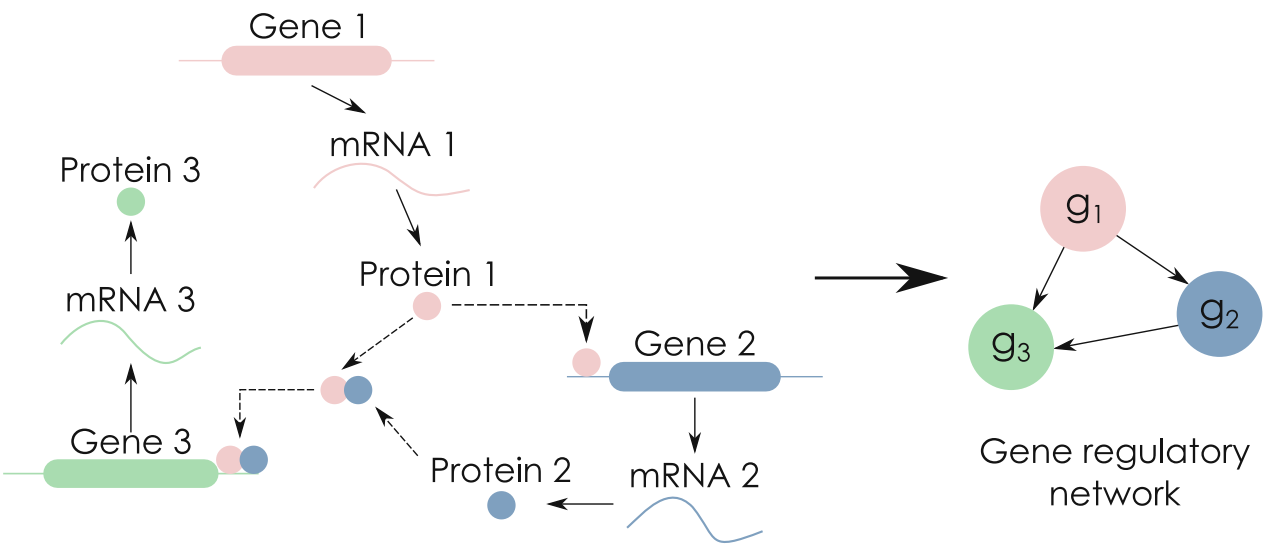
\includegraphics[scale = 0.4]{Figures/Intro/network.PNG}
	    \caption{Illustration schématique d'un réseau de régulation entre 3 gènes \scriptsize \cite{sanguinetti2019gene}}
	    \label{fig:my_label}
	\end{figure}
\end{frame}



\begin{frame}{Exemple de réseau de régulation chez Arabidopsis}

\begin{center}
    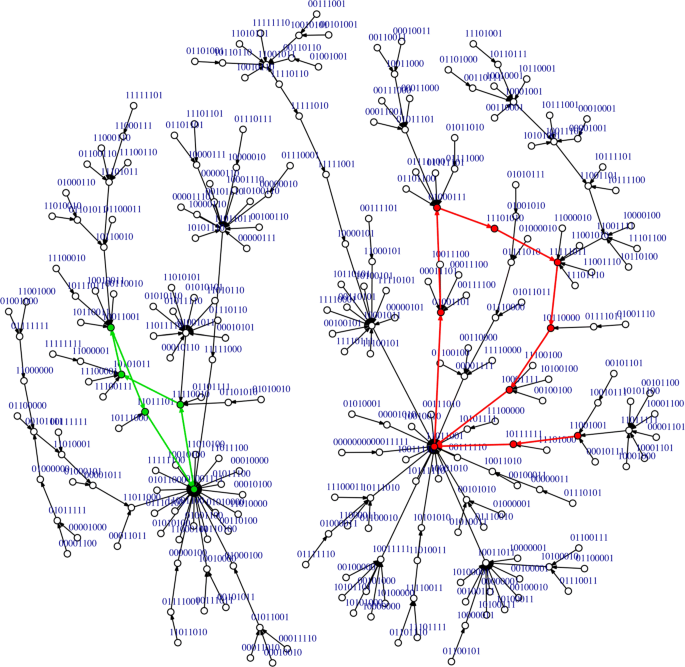
\includegraphics[scale = 0.27]{Figures/Intro/arabidopsis_gene_network.png} 
\end{center}

\vspace{-0.5cm}

\begin{tiny}
Timmermann, T., González, B. \& Ruz, G.A. Reconstruction of a gene regulatory network of the induced systemic resistance defense response in Arabidopsis using boolean networks. BMC Bioinformatics 21, 142 (2020). 
\end{tiny}
%https://doi.org/10.1186/s12859-020-3472-3

\end{frame}

	
	
\begin{frame}{Exemple de réseau de régulation chez Arabidopsis}
\begin{center}
    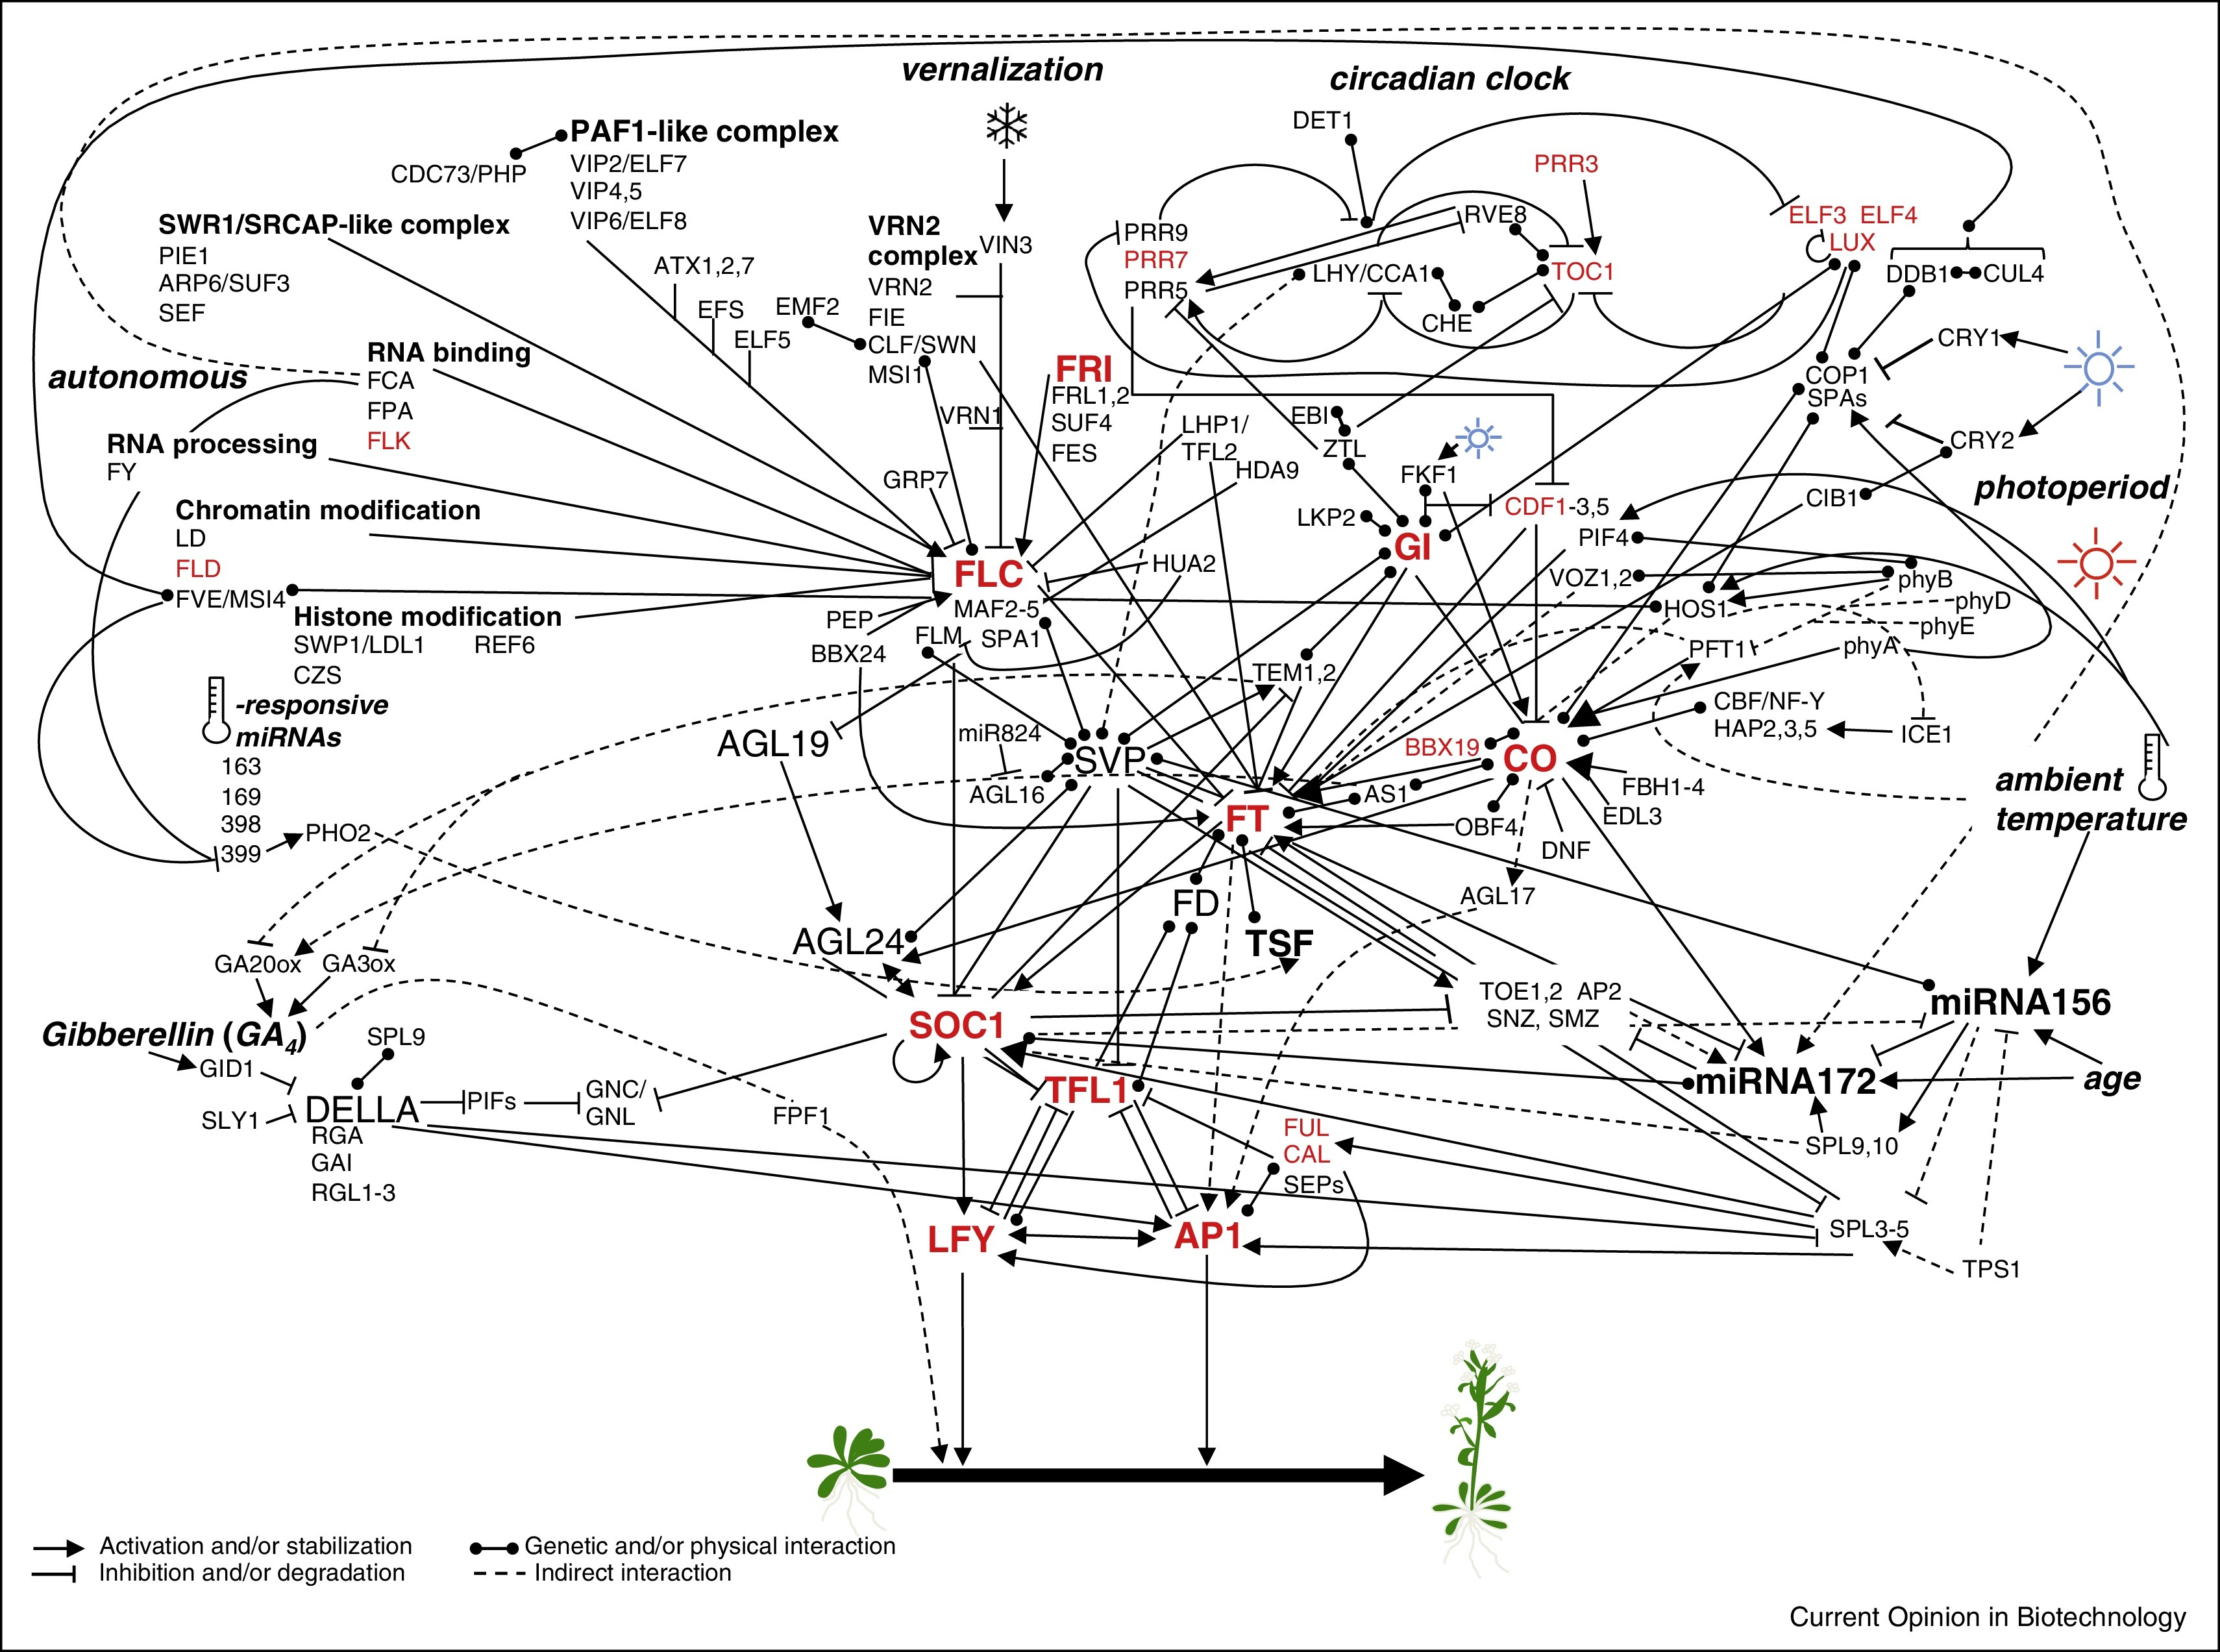
\includegraphics[scale = 0.45]{Figures/Intro/flowering-network-in-arabidopsis.jpeg}
 \end{center}
 
\begin{tiny}
    Flowering time gene network with known genetic and epigenetic regulators in Arabidopsis thaliana.\\
    Blümel, et al., 2015, Current Opinion in Biotechnology
    \end{tiny}
\end{frame}

	
	
\begin{frame}
\frametitle{Utilisation des réseaux en génomique fonctionnelle}
\vspace{-0.1cm}
\hspace{6.3cm}	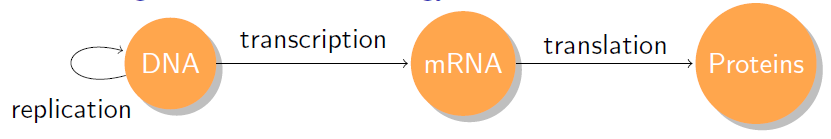
\includegraphics[width=5cm]{Figures/Intro/DogmeBM.png} 
\vspace{-0.5cm}		
\begin{itemize}
\item Différents domaines d'application
\begin{itemize}
\item \textcolor{Periwinkle}{Biologie fondamentale}
\begin{itemize}
\item Fonction et interaction des gènes et proteines (annotations, base de données), Machinerie cellulaire
\end{itemize}
\item \textcolor{Periwinkle}{Santé, Médecine}
\begin{itemize}
\item Diagnostique (ex: type de tumeur cancéreuse), Pronostique (ex: analyse de survie), Thérapie (ex: prédiction de la réponse à un traitement, médecine personnlisée)
\end{itemize}
\item \textcolor{Periwinkle}{Biologie végétale} 
\begin{itemize}
\item Agriculture, alimentation
\end{itemize}
\end{itemize}

\item Différents niveaux d'observation
\begin{itemize}\small
\item \textcolor{Periwinkle}{Génome} : analyse de séquence (ex: détection de motifs)
\item \textcolor{Periwinkle}{Transcriptome} : quantité d'ARN messager
\item \textcolor{Periwinkle}{Protéome} : quantité de protéines / interactions et fonctions des protéines
\end{itemize}
	
\end{itemize}
\end{frame}


	\begin{frame}{Données pour l'inférence d'un GRN}
\begin{itemize}
   \item Les \textbf{données de séquences génomiques} ... (PWM, JASPAR, ...)
    \pause
    \item Les \textbf{données de fixation} des régulateurs sur les promoteurs cibles sont très utiles, cependant : 
    
    \begin{itemize}\scriptsize
        \item Leur génération est relativement chère, contraignante donc faisable sur un \textbf{nombre très restreint de régulateurs}. 
        \item La fixation d'un TF n'implique pas régulation, et la régulation n'implique pas la fixation. (Interactions distantes, transcientes, coopération...)
    \end{itemize}
      \pause
    
    \item Les \textbf{données d'expression} :
    
    \begin{itemize}\scriptsize
        \item Leur mesure tous les gènes d'un organisme est plus accessible, via puces ou RNA-Seq.
        \item L'expression est une conséquence indirecte, il faut donc "démêler", "deviner", ce qui est de la régulation, ou ce qui est de la co-expression fortuite ou induite par des régulations communes
        \end{itemize}
\end{itemize}
	\end{frame}
	
	
	

\begin{frame}{Données pour l'inférence d'un GRN}
    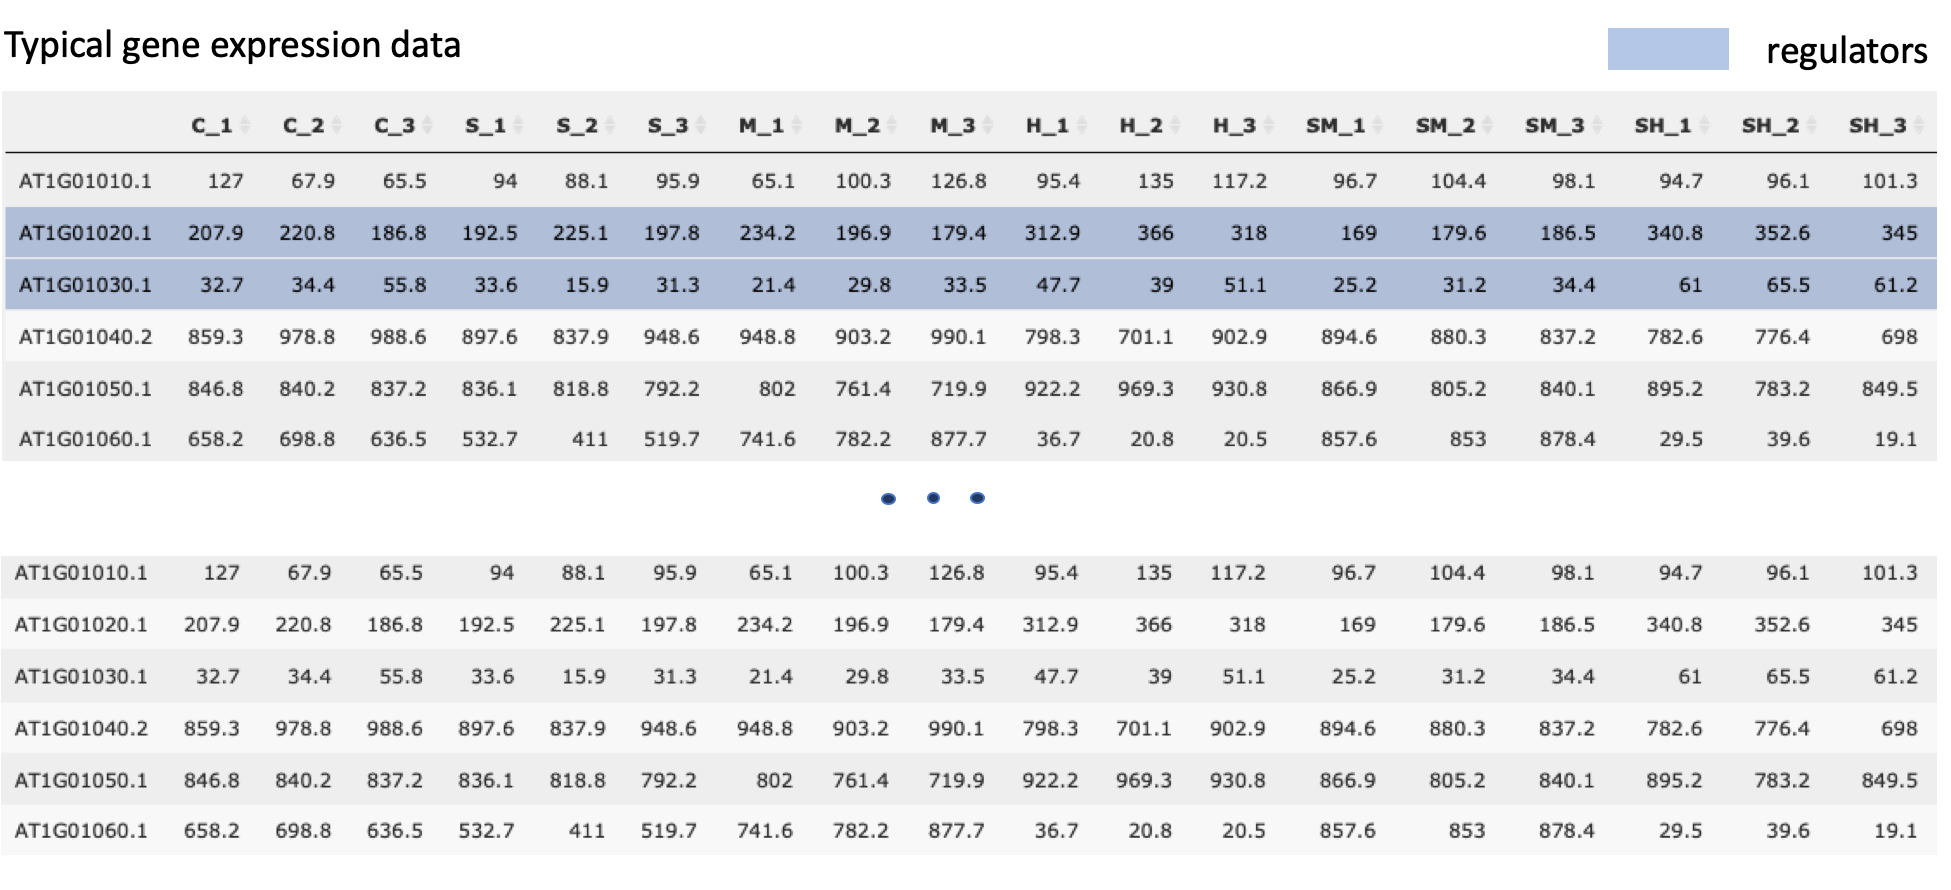
\includegraphics[scale = 0.17]{Figures/Intro/expression_data.png}
\end{frame}

	
\subsection{Réseau de co-expression vs réseau de régulation}



\begin{frame}
\frametitle{Modélisation et inférence ? }
\vspace{-0.1cm}
\begin{center}
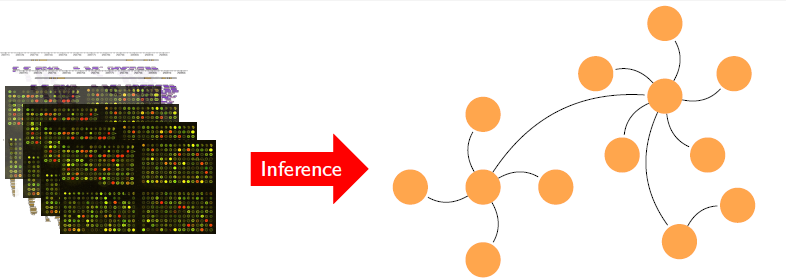
\includegraphics[width=9cm]{Figures/Intro/inference.png}
\end{center}
\vspace{-0.15cm}
\begin{itemize}\small
\item Que représentent les noeuds ? les arêtes ?
\item Biologiquement ? Statistiquement ? 
\item Est-ce que les arêtes sont orientées ? (causalité)
\item Le réseau est-il statique ? dynamique ? 
\item Comment les données ont-elles été générées ? (temporelles (time course), différentes conditions expérimentales (steady state), réplicats)
\end{itemize}

\end{frame}

\begin{frame}
\frametitle{Modélisation et inférence ? }
\vspace{-0.1cm}
\begin{center}
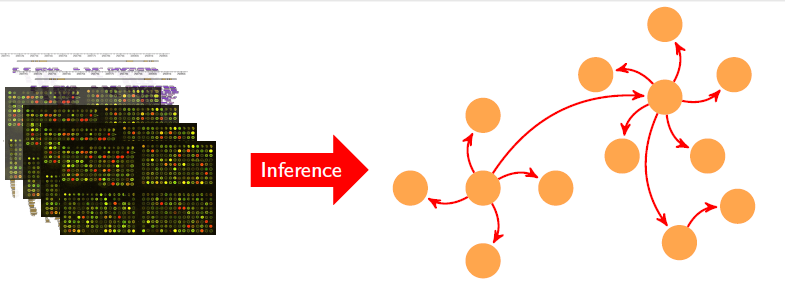
\includegraphics[width=9cm]{Figures/Intro/inference_oriente.png}
\end{center}
\vspace{-0.15cm}
\begin{itemize}\small
\item Que représentent les noeuds ? les arêtes ?
\item Biologiquement ? Statistiquement ? 
\item Est-ce que les arêtes sont orientées ? (causalité)
\item Le réseau est-il statique ? dynamique ? 
\item Comment les données ont-elles été générées ? (temporelles (time course), différentes conditions expérimentales (steady state), réplicats)
\end{itemize}

\end{frame}

\begin{frame}{Le problème de la grande dimension (p $>$ n) }


\small \textbf{Si les données d'expression à disposition contiennent $p$ gènes et $n$ conditions expérimentales:}

\begin{itemize} \small 
    \item les données à disposition sont de l'ordre de $n*p$
    \item les données que nous aimerions obtenir, c.a.d les liens entre les gènes, sont de l'ordre de  $p*p$
\end{itemize}

Si $p>n$, le volume d'information que nous essayons de reconstruire est plus grand que le volume d'information que nous avons à disposition! Et c'est très souvent le cas.

\center
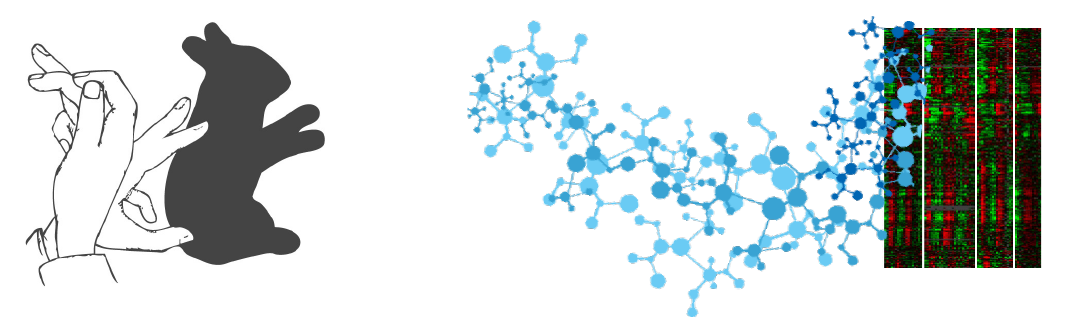
\includegraphics[scale = 0.2]{Figures/Intro/shadowplay.png}
    
\end{frame}

\begin{frame}{Régulation $\neq$ Co-expression}
	\begin{columns}[T] % align columns
        \begin{column}{.45\textwidth}
            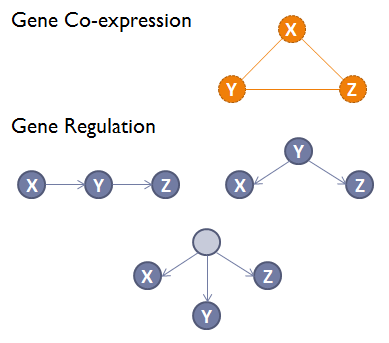
\includegraphics[scale = 0.65]{Figures/Intro/Gene_co-expression_vs_regulation.png}
        \end{column}
        \hfill%
        \begin{column}{.45\textwidth}
            \textcolor{orange}{\textbf{Réseau de co-expression:}}
                    \begin{itemize}
                      \item Arêtes non orientées
                      \item Arêtes reliant tous les types de gènes
                    \end{itemize}
            \vspace{0.5cm}
            \textcolor{Periwinkle}{\textbf{Réseau de régulation:}}
            \begin{itemize}
                  \item Arêtes orientées
                  \item Arêtes partant des gènes régulateurs vers les gènes cibles
            \end{itemize}
        \end{column}%
\end{columns}
\end{frame}
	
	
\begin{frame}{Signification d'un réseau de régulation}
\begin{itemize}
    \item Les réseaux de régulation sont \textbf{plus contraints} que les réseaux de co-expression, et portent une signification biologique \textbf{plus précise}
    \item Les réseaux de régulation recherchent plus de \textbf{causalité} dans l'explication des dépendances transcriptionnelles
    \onslide<2> 
    \vspace{0.5cm}
    \begin{alertblock}{Attention aux interprétations}
    La causalité reste toute fois difficile à atteindre
    \end{alertblock}
    
    
\end{itemize}
	\end{frame}


	


